\documentclass[tikz,border=0pt]{standalone}
\usepackage{xcolor}
\usetikzlibrary{calc}
% Palette: Sam_Comm_final.png by eye, and the drones and raiders.
\definecolor{ink}{HTML}{3B2340}
\definecolor{sky}{HTML}{EFC46A}
\definecolor{skyhi}{HTML}{F5DA92}
\definecolor{skylow}{HTML}{E9B060}
\definecolor{cloud}{HTML}{F2D58A}
\definecolor{paper}{HTML}{FBEFD0}
\definecolor{cream}{HTML}{FFF6E0}
\definecolor{white}{HTML}{FFFFFF}
\definecolor{wallA}{HTML}{E88A73}
\definecolor{wallB}{HTML}{EE9F7E}
\definecolor{wallC}{HTML}{E47A7E}
\definecolor{wallD}{HTML}{F0B07E}
\definecolor{wallE}{HTML}{D9765F}
\definecolor{wallF}{HTML}{E99A8A}
\definecolor{greenA}{HTML}{8DBB7E}
\definecolor{greenB}{HTML}{6FA77A}
\definecolor{greenC}{HTML}{A9C97F}
\definecolor{greenD}{HTML}{5E9C6A}
\definecolor{greenE}{HTML}{4A8060}
\definecolor{sage}{HTML}{9DB98A}
\definecolor{sagedark}{HTML}{6F8F66}
\definecolor{sagelight}{HTML}{C2D6A6}
\definecolor{window}{HTML}{F6E7A0}
\definecolor{windark}{HTML}{8C5A64}
\definecolor{metal}{HTML}{8D9A93}
\definecolor{metaldark}{HTML}{5E6B66}
\definecolor{metallight}{HTML}{B9C4BC}
\definecolor{wood}{HTML}{B9835A}
\definecolor{wooddark}{HTML}{8C5A3C}
\definecolor{woodlight}{HTML}{D9A66F}
\definecolor{stone}{HTML}{E7C9A0}
\definecolor{stonedark}{HTML}{C9A47E}
\definecolor{concrete}{HTML}{D8C3A4}
\definecolor{concretedark}{HTML}{B8A084}
\definecolor{asphalt}{HTML}{8E7A86}
\definecolor{asphaltdark}{HTML}{6E5C68}
\definecolor{roadline}{HTML}{F6E7A0}
\definecolor{kerb}{HTML}{D8B48C}
\definecolor{red}{HTML}{E0483E}
\definecolor{redlight}{HTML}{F27A6A}
\definecolor{gold}{HTML}{FFB000}
\definecolor{goldlight}{HTML}{FFD54F}
\definecolor{teal}{HTML}{4FA3A0}
\definecolor{tealdark}{HTML}{3C8582}
\definecolor{magenta}{HTML}{FF2E88}
\definecolor{cyan}{HTML}{13CFE3}
\definecolor{violet}{HTML}{8A5BD6}
\definecolor{orange}{HTML}{F2803A}
\definecolor{pink}{HTML}{F48FB1}
\definecolor{glow}{HTML}{4FE6E0}
\definecolor{glowhi}{HTML}{C8FFF9}
\definecolor{hot}{HTML}{FF6A1A}
\definecolor{hothi}{HTML}{FFD07A}
\definecolor{armour}{HTML}{7E7A86}
\definecolor{armourdark}{HTML}{5A5466}
\definecolor{armourlight}{HTML}{A8A2B0}
\definecolor{wasp}{HTML}{E0A82E}
\definecolor{waspdark}{HTML}{B07E1A}
\definecolor{moth}{HTML}{F2E6C8}
\definecolor{mothdark}{HTML}{D2C09A}
\definecolor{hornet}{HTML}{3C8582}
\definecolor{hornetdark}{HTML}{2C6260}
\definecolor{warden}{HTML}{E47A7E}
\definecolor{wardendark}{HTML}{B85A62}
\definecolor{tick}{HTML}{8DBB7E}
\definecolor{tickdark}{HTML}{5E8A5A}
\definecolor{strider}{HTML}{D9765F}
\definecolor{striderdark}{HTML}{A8543F}
\definecolor{jacket}{HTML}{6FA77A}
\definecolor{jacketb}{HTML}{4FA3A0}
\definecolor{jacketc}{HTML}{E88A73}
\definecolor{jacketd}{HTML}{F0B07E}
\definecolor{skin}{HTML}{F2C49A}
\definecolor{skinb}{HTML}{C98C6A}
\definecolor{skinc}{HTML}{8C5A3C}
\definecolor{hair}{HTML}{3B2340}
\definecolor{goo}{HTML}{B6E35A}
\definecolor{goodark}{HTML}{7FB23A}
\newcommand{\Ink}{1.6pt}
\tikzset{inked/.style={draw=ink, line width=\Ink, line join=round, line cap=round}}
\begin{document}
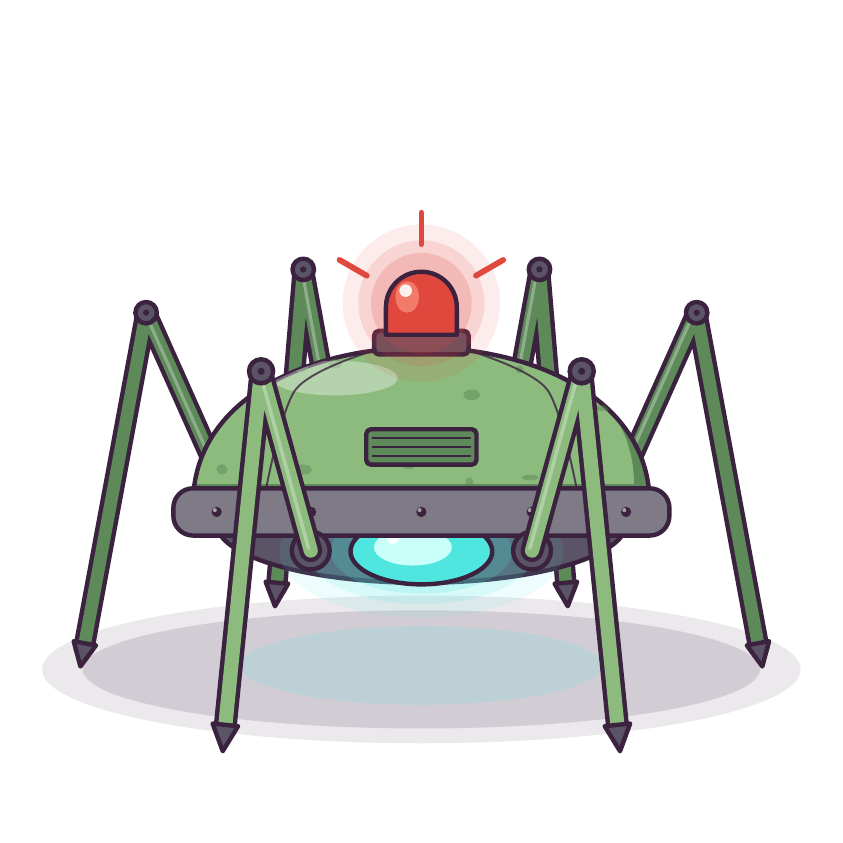
\begin{tikzpicture}
\clip (0,0) rectangle (10,10);
\begin{scope}[shift={(0,0)}, scale=1]
\fill[ink, opacity=0.10] (5,1.85) ellipse (4.816 and 0.938);
\fill[ink, opacity=0.14] (5,1.85) ellipse (4.3 and 0.75);
\fill[glow, opacity=0.16] (5.0,1.9) ellipse (2.3 and 0.5);
\draw[ink, line width=7.752pt, line cap=round, line join=round] (7.413,3.954) -- (8.496,6.38) -- (9.284,2.132);
\draw[tickdark, line width=4.552pt, line cap=round, line join=round] (7.413,3.954) -- (8.496,6.38) -- (9.284,2.132);
\draw[white, opacity=0.3, line width=1.138pt, line cap=round] (7.389,3.978) -- (8.472,6.404);
\filldraw[inked,fill=armourdark] (8.496,6.38) circle (0.136);
\fill[ink] (8.496,6.38) circle (0.04);
\filldraw[inked,fill=armourdark] (9.416,2.208) -- (9.33,1.887) -- (9.133,2.155) -- cycle;
\draw[ink, line width=7.752pt, line cap=round, line join=round] (6.035,4.394) -- (6.5,6.93) -- (6.838,2.902);
\draw[tickdark, line width=4.552pt, line cap=round, line join=round] (6.035,4.394) -- (6.5,6.93) -- (6.838,2.902);
\draw[white, opacity=0.3, line width=1.138pt, line cap=round] (6.011,4.418) -- (6.476,6.954);
\filldraw[inked,fill=armourdark] (6.5,6.93) circle (0.136);
\fill[ink] (6.5,6.93) circle (0.04);
\filldraw[inked,fill=armourdark] (6.978,2.963) -- (6.859,2.652) -- (6.691,2.939) -- cycle;
\draw[ink, line width=7.752pt, line cap=round, line join=round] (3.965,4.394) -- (3.5,6.93) -- (3.162,2.902);
\draw[tickdark, line width=4.552pt, line cap=round, line join=round] (3.965,4.394) -- (3.5,6.93) -- (3.162,2.902);
\draw[white, opacity=0.3, line width=1.138pt, line cap=round] (3.941,4.418) -- (3.476,6.954);
\filldraw[inked,fill=armourdark] (3.5,6.93) circle (0.136);
\fill[ink] (3.5,6.93) circle (0.04);
\filldraw[inked,fill=armourdark] (3.309,2.939) -- (3.141,2.652) -- (3.022,2.963) -- cycle;
\draw[ink, line width=7.752pt, line cap=round, line join=round] (2.587,3.954) -- (1.504,6.38) -- (0.716,2.132);
\draw[tickdark, line width=4.552pt, line cap=round, line join=round] (2.587,3.954) -- (1.504,6.38) -- (0.716,2.132);
\draw[white, opacity=0.3, line width=1.138pt, line cap=round] (2.563,3.978) -- (1.48,6.404);
\filldraw[inked,fill=armourdark] (1.504,6.38) circle (0.136);
\fill[ink] (1.504,6.38) circle (0.04);
\filldraw[inked,fill=armourdark] (0.867,2.155) -- (0.67,1.887) -- (0.584,2.208) -- cycle;
\filldraw[inked,fill=armourdark] (5,3.7) ellipse (2.6 and 0.75);
\fill[glow, opacity=0.1] (5,3.35) ellipse (1.8 and 0.84);
\fill[glow, opacity=0.14] (5,3.35) ellipse (1.44 and 0.672);
\fill[glow, opacity=0.2] (5,3.35) ellipse (1.152 and 0.538);
\filldraw[inked,fill=glow] (5,3.35) ellipse (0.9 and 0.42);
\fill[glowhi]  (4.892,3.4) ellipse (0.495 and 0.231);
\fill[white, opacity=0.9] (4.64,3.518) circle (0.076);
\fill[tickdark] (2.1,3.95) .. controls (2.1,6.6) and (7.9,6.6) .. (7.9,3.95) -- cycle;
\begin{scope}\clip (2.1,3.95) .. controls (2.1,6.6) and (7.9,6.6) .. (7.9,3.95) -- cycle;
\begin{scope}[shift={(-0.2,0.25)}]\fill[tick] (2.1,3.95) .. controls (2.1,6.6) and (7.9,6.6) .. (7.9,3.95) -- cycle;\end{scope}
\end{scope}
\draw[inked] (2.1,3.95) .. controls (2.1,6.6) and (7.9,6.6) .. (7.9,3.95) -- cycle;
\begin{scope}\clip (2.1,3.95) .. controls (2.1,6.6) and (7.9,6.6) .. (7.9,3.95) -- cycle;
\begin{scope}\clip (2.1,3.95) .. controls (2.1,6.6) and (7.9,6.6) .. (7.9,3.95) -- cycle;
\fill[tickdark, opacity=0.5] (5.639,5.335) ellipse (0.106 and 0.068);
\fill[tickdark, opacity=0.5] (6.247,5.66) ellipse (0.052 and 0.049);
\fill[tickdark, opacity=0.5] (7.305,5.168) ellipse (0.113 and 0.035);
\fill[tickdark, opacity=0.5] (4.839,4.444) ellipse (0.088 and 0.053);
\fill[tickdark, opacity=0.5] (2.468,4.39) ellipse (0.07 and 0.067);
\fill[tickdark, opacity=0.5] (6.382,4.287) ellipse (0.106 and 0.036);
\fill[tickdark, opacity=0.5] (5.611,4.228) ellipse (0.05 and 0.065);
\fill[tickdark, opacity=0.5] (3.489,4.388) ellipse (0.119 and 0.065);
\fill[tickdark, opacity=0.5] (3.904,5.731) ellipse (0.088 and 0.057);
\fill[tickdark, opacity=0.5] (3.465,5.694) ellipse (0.098 and 0.069);
\end{scope}
\fill[white, opacity=0.35] (3.9,5.55) ellipse (0.8 and 0.22);
\end{scope}
\draw[ink, line width=0.7pt, line cap=round, line join=round, opacity=0.8] plot[smooth, tension=0.5] coordinates {(3,4) (3.4,5.4) (4.4,5.9)};
\draw[ink, line width=0.7pt, line cap=round, line join=round, opacity=0.8] plot[smooth, tension=0.5] coordinates {(7,4) (6.6,5.4) (5.6,5.9)};
\filldraw[inked,fill=armour,rounded corners=0.25cm] (1.85,3.55) rectangle (8.15,4.15);
\fill[ink] (2.4,3.85) circle (0.065);
\fill[white, opacity=0.55] (2.377,3.873) circle (0.026);
\fill[ink] (3.6,3.85) circle (0.065);
\fill[white, opacity=0.55] (3.577,3.873) circle (0.026);
\fill[ink] (5,3.85) circle (0.065);
\fill[white, opacity=0.55] (4.977,3.873) circle (0.026);
\fill[ink] (6.4,3.85) circle (0.065);
\fill[white, opacity=0.55] (6.377,3.873) circle (0.026);
\fill[ink] (7.6,3.85) circle (0.065);
\fill[white, opacity=0.55] (7.577,3.873) circle (0.026);
\filldraw[inked,fill=tickdark,rounded corners=0.06cm] (4.3,4.45) rectangle (5.7,4.9);
\draw[ink, line width=0.8pt, line cap=round] (4.38,4.562) -- (5.62,4.562);
\draw[ink, line width=0.8pt, line cap=round] (4.38,4.675) -- (5.62,4.675);
\draw[ink, line width=0.8pt, line cap=round] (4.38,4.788) -- (5.62,4.788);
\filldraw[inked,fill=armourdark,rounded corners=0.06cm] (4.4,5.85) rectangle (5.6,6.15);
\fill[red, opacity=0.1] (5,6.5) ellipse (1 and 1);
\fill[red, opacity=0.14] (5,6.5) ellipse (0.8 and 0.8);
\fill[red, opacity=0.2] (5,6.5) ellipse (0.64 and 0.64);
\filldraw[inked, fill=red] (4.55,6.1) -- (4.55,6.45) arc[start angle=180, end angle=0, radius=0.45] -- (5.45,6.1) -- cycle;
\fill[redlight] (4.82,6.58) ellipse (0.15 and 0.2);
\fill[white, opacity=0.9] (4.8,6.66) circle (0.08);
\draw[red, line width=2.08pt, line cap=round] (5.693,6.85) -- (6.039,7.05);
\draw[red, line width=2.08pt, line cap=round] (5,7.25) -- (5,7.65);
\draw[red, line width=2.08pt, line cap=round] (4.307,6.85) -- (3.961,7.05);
\filldraw[inked,fill=armourdark] (3.595,3.359) circle (0.24);
\draw[ink, line width=8.322pt, line cap=round, line join=round] (3.595,3.359) -- (2.964,5.636) -- (2.505,1.09);
\draw[tick, line width=5.122pt, line cap=round, line join=round] (3.595,3.359) -- (2.964,5.636) -- (2.505,1.09);
\draw[white, opacity=0.3, line width=1.28pt, line cap=round] (3.568,3.386) -- (2.937,5.663);
\filldraw[inked,fill=armourdark] (2.964,5.636) circle (0.153);
\fill[ink] (2.964,5.636) circle (0.045);
\filldraw[inked,fill=armourdark] (2.672,1.129) -- (2.477,0.811) -- (2.349,1.162) -- cycle;
\filldraw[inked,fill=armourdark] (6.405,3.359) circle (0.24);
\draw[ink, line width=8.322pt, line cap=round, line join=round] (6.405,3.359) -- (7.036,5.636) -- (7.495,1.09);
\draw[tick, line width=5.122pt, line cap=round, line join=round] (6.405,3.359) -- (7.036,5.636) -- (7.495,1.09);
\draw[white, opacity=0.3, line width=1.28pt, line cap=round] (6.378,3.386) -- (7.009,5.663);
\filldraw[inked,fill=armourdark] (7.036,5.636) circle (0.153);
\fill[ink] (7.036,5.636) circle (0.045);
\filldraw[inked,fill=armourdark] (7.651,1.162) -- (7.523,0.811) -- (7.328,1.129) -- cycle;
\end{scope}
\end{tikzpicture}
\end{document}
